\documentclass[12pt]{article}

%\RequirePackage{scrpage2} %% obsolete --> use scrlayer-scrpage instead if needed
\RequirePackage[utf8]{inputenc}
\RequirePackage[T1]{fontenc}
\RequirePackage[ngerman]{babel}
\RequirePackage[german]{babelbib}
\RequirePackage{microtype}
\RequirePackage{pifont}
\RequirePackage{lmodern}
\RequirePackage{latexsym,amssymb,amsmath,mathdots}
\RequirePackage{wasysym}
% \RequirePackage{txfonts}
% \RequirePackage[scaled=.9]{helvet}
\RequirePackage{xspace}
\RequirePackage[pdfborder={0 0 0}]{hyperref}
\RequirePackage{graphicx}
\RequirePackage{tikz}
\usetikzlibrary{automata,positioning,arrows.meta,shapes,calc,fit}
\RequirePackage{ifthen}
\RequirePackage{rotating}

\RequirePackage{chngcntr}
\counterwithout{figure}{section}
\renewcommand\thefigure{\arabic{figure}}
\counterwithout{equation}{section}

%\DeclareFontShape{U}{wasy}{b}{n}{%
%<->wasyb10%
%}{}

\wasyfamily
\DeclareFontShape{U}{wasy}{b}{n}{ <-10> ssub * wasy/m/n
 <10> <10.95> <12> <14.4> <17.28> <20.74> <24.88>wasyb10 }{}

\renewcommand\thepart{\arabic{part}}
\renewcommand\partname{Kapitel}

\renewcommand\floatpagefraction{.99}
\renewcommand\topfraction{.99}
\renewcommand\bottomfraction{.99}
\renewcommand\textfraction{.01}

\pgfdeclarelayer{background}
\pgfdeclarelayer{foreground}
\pgfsetlayers{background,main,foreground}

\hyphenation{Konzept-inklusion}

\newcommand{\textbfsf}[1]{\textbf{\textsf{#1}}}
\newcommand{\textsfbf}[1]{\textbf{\textsf{#1}}}

% Beweisumgebung
\newcommand{\qedsymbol}{\ding{111}}
\newcommand{\qedhere}{\hspace*{\fill}\qedsymbol}
\newcommand{\quasiqedhere}{\hspace*{\fill}(\qedsymbol)}
\newenvironment{beweis}{%
  \par\medskip\noindent
  \textup{\textsfbf{Beweis.}}
}{%
%   \hspace*{\fill}\qedsymbol
  \par\smallskip\noindent
}

% ----- Frakturbuchstaben -----
\newcommand{\Amf}{\ensuremath{\mathfrak{A}}\xspace}
\newcommand{\Bmf}{\ensuremath{\mathfrak{B}}\xspace}
\newcommand{\Imf}{\ensuremath{\mathfrak{I}}\xspace}
\newcommand{\Nmf}{\ensuremath{\mathfrak{N}}\xspace}

% ----- kalligrafische Buchstaben -----
\newcommand{\Amc}{\ensuremath{\mathcal{A}}\xspace}
\newcommand{\Bmc}{\ensuremath{\mathcal{B}}\xspace}
\newcommand{\Fmc}{\ensuremath{\mathcal{F}}\xspace}
\newcommand{\Gmc}{\ensuremath{\mathcal{G}}\xspace}
\newcommand{\Imc}{\ensuremath{\mathcal{I}}\xspace}
\newcommand{\Jmc}{\ensuremath{\mathcal{J}}\xspace}
\newcommand{\Kmc}{\ensuremath{\mathcal{K}}\xspace}
\newcommand{\Lmc}{\ensuremath{\mathcal{L}}\xspace}
\newcommand{\Omc}{\ensuremath{\mathcal{O}}\xspace}
\newcommand{\Pmc}{\ensuremath{\mathcal{P}}\xspace}
\newcommand{\Smc}{\ensuremath{\mathcal{S}}\xspace}
\newcommand{\Tmc}{\ensuremath{\mathcal{T}}\xspace}
\newcommand{\Umc}{\ensuremath{\mathcal{U}}\xspace}

% ----- Carstens phi-Abkürzung -----
\newcommand{\vp}{\ensuremath{\varphi}\xspace}

% ----- Makros für lineare Strukturen und deren Labels -----
\newcommand{\linstruc}[1]{%
  \node[state] (elem0) {0};
  \foreach \x [remember=\x as \lastx (initially 0)] in {1,...,#1} {
      \node[state] (elem\x) [right=of elem\lastx] {\x};
      \path[->] (elem\lastx) edge node[above] {$s$} (elem\x);
  };

  \path[->] (elem#1) edge[loop right] node[right] {$s$} ();
}

% 1st param: location of label w.r.t. to element (default: above)
% 2nd param: distance to element
% 3rd param: element name
% 4th param: alignment among labels
% 5th param: label text (without "tabular")
\newcommand{\linstruclab}[5][above]{%
  \node [#1=#2 of elem#3] {\begin{tabular}{@{}#4@{}}#5\end{tabular}};
}

\renewcommand{\Vec}[1]{\ensuremath{\overrightarrow{#1}}}

\newcommand{\bspnr}[1]{{\footnotesize\textsf{#1}}}

\newcommand{\auf}{\ensuremath{\langle}}
\newcommand{\zu}{\ensuremath{\rangle}}

\newcommand*\circled[1]{\tikz[baseline=(char.base)]{
            \node[shape=circle,draw,inner sep=1pt,line width = .8pt] (char) {{\small #1}};}}

\newcommand{\term}[1]{\textsf{#1}}

\newcommand{\DL}[1]{\ensuremath{\mathcal{#1}}}
\newcommand{\ALC}{\DL{ALC}\xspace}
\newcommand{\ALCI}{\DL{ALCI}\xspace}
\newcommand{\ALCQ}{\DL{ALCQ}\xspace}
\newcommand{\ALCQI}{\DL{ALCQI}\xspace}

\newcommand{\qnrgeq}[3]{\ensuremath{(\mathord{\geqslant}#1\,#2.#3)}}
\newcommand{\qnrleq}[3]{\ensuremath{(\mathord{\leqslant}#1\,#2.#3)}}

\newcommand{\parI}{\par\smallskip}
\newcommand{\parII}{\par\medskip}
\newcommand{\parIII}{\par\bigskip}

\newenvironment{tboxarray}{%
  \renewcommand{\arraystretch}{1.2}
  \begin{array}{@{}r@{~~}r@{~~}c@{~~}l@{~~}l@{}}
}{%
  \end{array}
} 

\begin{document}
 
\title{Beschreibungslogik | Übung 04}
\author{D. Marschner, A. Mahdavi\\
\href{mailto:alma@uni-bremen.de}{alma@uni-bremen.de}\\
\href{mailto:mail@dennis-marschner.de}{mail@dennis-marschner.de}
}
\date{}
\maketitle
\section*{Aufgabe 1)}
\subsection*{a)}
Wahr, intuitiv ist jeder semantische Typ auch ein syntaktischer Typ, umgekehrt ist das nicht der Fall. Das Ziel der Typelimination ist es, diejenigen syntaktischen Typen zu eliminieren, die im Modell der TBox nicht zu finden sind.
\subsection*{b)}
Falsch! Schlussfolgerung Probleme Äquivalenz, Subsumtion und Konzept Erfüllbarkeit in Bezug auf T-Boxen sind in wechselseitiger Abhängigkeit. Man kann sie Polynomiell aufeinander reduzieren. 
Vgl: Lemma 2.9
\subsection*{c)}
Wahr, Der Tableau-Algorithmus benötigt im Worst-Case eine 3-fache exponentielle Laufzeit, aber die Typelimination benötigt  im Worst- sowie Best Case nur eine exponentielle Laufzeit.
\subsection*{d)}
Falsch! Es gibt nur $2^n$ viele Typen und nach jedem Schritt der repeat-Schleife wird mindestens ein Typ eliminiert. Schleife terminiert nach maximal $2^n$ Durchläufen. Somit ist ein Backtracking nicht notwendig. Vgl. auch Folie 5.13.
\subsection*{e)}
Wahr, denn bei der Typelimination generiert man alle Typen für $C_0$ und $\Tmc$ (exponentiell viele), wobei jeder Typ $t$ Teilmenge von $sub(C_0, \Tmc)$ ist. $sub(C_0, \Tmc)$ ist schon eine Art “Absorption”, da die Menge $sub(C_0,\Tmc)$ keine doppelten Konzepte enthält. Also die meisten “doppelten”,”unnötigen” Konzepte, die man durch Absorption verwerfen könnte, werden durch die Generierung der Sub-Menge per Definition ohnehin entfernt.
\subsection*{f)}
Wahr!  Es kann zwar ein $\Imc$ geben mit: \{$t_{\Imc}(d) | d \in \Delta^{\Imc} $\}  $\subseteq \Gamma$\\
aber der zweite Teil: $t = t_{\Imc}(d_0)$ für ein $d_0 \in \Delta^{\Imc} $ ist unmöglich erfüllbar, da intuitiv $t(d_0)$ mindestens eine Existenz Restriktion hat, für die es keinen r-Nachfolger (Zeuge) gibt. Somit wird es nie eine Interpretation $\Imc$ geben, für die gilt:  $t = t_{\Imc}(d_0)$ für ein $d_0 \in \Delta^{\Imc} $.  Vgl: Definition 5.3 schlechter Typ.


\section*{Aufgabe 2)}
\subsection*{a)}
$C_0$ = $\exists r. \neg A$ erfüllbar bzgl. $\Tmc$ = $\{\forall r.A \sqsubseteq A, A \sqsubseteq \bot, \forall r.A \sqsubseteq \exists r.A\}$\\
\\
$\Tmc$ in NNF bringen:
%
\begin{flalign*}
\Tmc & = \{\forall r.A \sqsubseteq A, A \sqsubseteq \bot, \forall r.A \sqsubseteq \exists r.A\}\\
&= \{\top \sqsubseteq (\neg \forall r.A \sqcup A) \sqcap (\neg A \sqcup \bot) \sqcap (\neg \forall r.A \sqcup \exists r.A) \}\\
&= \{\top \sqsubseteq (\exists r. \neg A \sqcup A) \sqcap \neg A \sqcap (\exists r. \neg A \sqcup \exists r.A) \}
\end{flalign*}
%
$\Tmc$ = $\{\top \sqsubseteq C_{\Tmc} \}$ mit $C_{\Tmc}$ = $\{(\exists r. \neg A \sqcup A) \sqcap \neg A \sqcap (\exists r. \neg A \sqcup \exists r.A) \}$\\
\\
$sub(C_0,\Tmc)$ generieren:
%
\begin{flalign*}
sub(C_0,\Tmc) & = \{\exists r. \neg A, C_{\Tmc}, \exists r. \neg A \sqcup A, \neg A, \exists r. \neg A \sqcup \exists r.A, A, \exists r.A\}
\end{flalign*}
%
Wegen $C_{\Tmc} \in t$ für jeden Typen $t$ für $C_0$ und $\Tmc$ und der Typ-Bedingung für $\sqcap$, muss jeder Typ die Menge $M = \{C_{\Tmc}, \exists r. \neg A \sqcup A, \neg A, \exists r. \neg A \sqcup \exists r.A \}$ enthalten.
Aufgrund der Regel-(1) von Definition 5.2 (Typ) und weil $\neg A \in sub(C_0,\Tmc)$ ist $A \not \in t$. Dadurch ergibt sich mit der $\sqcup$-Regel, dass $\exists r. \neg A \in t$ sein muss.\\
Somit ist $M = \{C_{\Tmc}, \exists r. \neg A \sqcup A, \neg A, \exists r. \neg A \sqcup \exists r.A, \exists r. \neg A\}$.
\\
Man kann sich also leicht überzeugen, dass es insgesamt zwei Typen für $C_0$ und $\Tmc$ gibt, nämlich:
%
\begin{flalign*}
& t_0 = M \cup \{\exists r.A \}\\
& t_1 = M
\end{flalign*}
%
Der Typ $t_0$ ist schlecht in der Menge aller Typen: für $\exists r.A \in t_0$ und $\exists r. \neg A \in t_0$ ist die Menge aus Definition 5.3 $\{A, \neg A\}$, aber kein Typ enthält sowohl $A$ als auch $\neg A$.\\
Der Typ $t_1$ ist nicht schlecht in der Menge aller Typen: für $\exists r. \neg A \in t_1$ ist die Menge aus Definition 5.3 $\{\neg A\}$, wobei $t_1$ selbst $\neg A$ enthält. Also $\neg A \in t_1 = t'$.\\
\\
Das Typeliminationsverfahren berechnet folgende Mengen:
%
\begin{flalign*}
%
\Gamma_0 & = \{t_0,t_1\}\\
%
\Gamma_1 & = \{t_1\}\\
%
\Gamma_2 & = \{t_1\}
%
\end{flalign*}
%
Der Algorithmus stoppt, weil $\Gamma_1$ = $\Gamma_2$.\\
Das Ergebnis ist $erfüllbar$, weil es ein $t = t_1 \in \Gamma_2$ gibt mit $C_0 = \exists r. \neg A \in t$.
%
\\\\
Model \Imc aus Beweis von Lemma 5.5:
%
\begin{center}
\parbox[t]{.5\linewidth}{%
\begin{tikzpicture}[%
>=Latex,baseline=.2pt,every state/.style={draw=black,thin,fill=black!10,inner sep=1mm,minimum size=8mm},every edge/.style={draw=black,thin}]
\node[state] (t0)                  {$t_0$};
\node [above left=0mm and 12mm of t0] {$\Imc$};
\path[->] (t0) edge [loop right] node[right] {$r$} ()        
;
\end{tikzpicture}%
}
\end{center}
%
\begin{flalign*}
%
\Delta^\Imc & = \{t_0\}\\
%
r^\Imc & = \{(t_0,t_0)\}\\
%
\end{flalign*}
%
Da $(C_0)^\Imc$ = $(\exists r. \neg A)^\Imc$ = $\{t_0\} \neq \emptyset$ ist $\Imc$ Modell von $C_0$.

\subsection*{b)}
$C_0$ = $\forall r. \forall r.A$ erfüllbar bzgl. $\Tmc$ = $\{\neg A \sqsubseteq B, A \sqsubseteq \neg B, \forall r.A \sqsubseteq \bot\}$\\
\\
$\Tmc$ in NNF bringen:
%
\begin{flalign*}
\Tmc & = \{\neg A \sqsubseteq B, A \sqsubseteq \neg B, \forall r.A \sqsubseteq \bot\}\\
&= \{\top \sqsubseteq (\neg \neg A \sqcup B) \sqcap (\neg A \sqcup \neg B) \sqcap (\neg \forall r.A \sqcup \bot) \}\\
&= \{\top \sqsubseteq ( A \sqcup B) \sqcap (\neg A \sqcup \neg B) \sqcap (\exists r. \neg A \sqcup \bot) \}\\
&= \{\top \sqsubseteq ( A \sqcup B) \sqcap (\neg A \sqcup \neg B) \sqcap \exists r. \neg A \}\\
\end{flalign*}
%
$\Tmc$ = $\{\top \sqsubseteq C_{\Tmc} \}$ mit $C_{\Tmc}$ = $\{( A \sqcup B) \sqcap (\neg A \sqcup \neg B) \sqcap \exists r. \neg A \}$\\
\\
$sub(C_0,\Tmc)$ generieren:
%
\begin{flalign*}
sub(C_0,\Tmc) & = \{\forall r. \forall r.A, C_{\Tmc},A \sqcup B,\neg A \sqcup \neg B, \exists r. \neg A, A, B, \neg A, \neg B,\forall r.A\}
\end{flalign*}
%
Wegen $C_{\Tmc} \in t$ für jeden Typen $t$ für $C_0$ und $\Tmc$ und der Typ-Bedingung für $\sqcap$, muss jeder Typ die Menge $M = \{C_{\Tmc},A \sqcup B,\neg A \sqcup \neg B, \exists r. \neg A \}$ enthalten.
Aufgrund der Regel-(1) von Definition 5.2 (Typ) und der $\sqcup$-Regel kann
man sich leicht überzeugen, dass es insgesamt vier Typen für $C_0$ und $\Tmc$ gibt, nämlich:
%
\begin{flalign*}
& t_0 = M \cup \{A, \neg B\}\\
& t_1 = M \cup \{\neg A, B\}\\
& t_2 = M \cup \{A, \neg B, \forall r. A\}\\
& t_3 = M \cup \{\neg A, B, \forall r. A\}\\
\end{flalign*}
%
Der Typ $t_0$ ist nicht schlecht in der Menge aller Typen: für $\exists r. \neg A \in t_0$ ist die Menge aus Definition 5.3 $\{\neg A\}$, wobei $\neg A \in t_1$. Also $\neg A \in t_1 = t'$.\\
\\
Der Typ $t_1$ ist nicht schlecht in der Menge aller Typen: für $\exists r. \neg A \in t_1$ ist die Menge aus Definition 5.3 $\{\neg A\}$, wobei $t_1$ selbst $\neg A$ enthält. Also $\neg A \in t_1 = t'$.\\
\\
Der Typ $t_2$ ist schlecht in der Menge aller Typen: für $\exists r. \neg A \in t_2$ und $\forall r. A \in t_2$ ist die Menge aus Definition 5.3 $\{\neg A, A\}$, aber kein Typ enthält sowohl $A$ als auch $\neg A$.\\
\\
Der Typ $t_3$ ist schlecht in der Menge aller Typen: für $\exists r. \neg A \in t_3$ und $\forall r. A \in t_3$ ist die Menge aus Definition 5.3 $\{\neg A, A\}$, aber kein Typ enthält sowohl $A$ als auch $\neg A$.\\
\\
Das Typeliminationsverfahren berechnet folgende Mengen:
%
\begin{flalign*}
%
\Gamma_0 & = \{t_0,t_1,t_2,t_3\}\\
%
\Gamma_1 & = \{t_0,t_1\}\\
%
\Gamma_2 & = \{t_0,t_1\}\\
%
\end{flalign*}
%
Der Algorithmus stoppt, weil $\Gamma_1$ = $\Gamma_2$.\\
Das Ergebnis ist $unerfüllbar$, weil es ein kein $t \in \Gamma_2$ gibt mit $C_0 = \forall r. \forall r. A \in t$.

\section*{Aufgabe 3)}
\subsection*{a)}
Es gibt keine Gewinnstrategie für Spieler 2, da Spieler 1 nach folgendem Vorgehen immer gewinnen kann.\\
\\
Wir teilen die gesamte Formel zunächst auf in $\varphi = A \lor B \lor C$ mit $A$ = $(p_1 \land p_2 \land \neg q_1), B = (p_3 \land p_4 \land \neg q_2), C = (\neg(p_1 \lor p_4) \land q_1 \land q_2)$.\\
\\
Spieler 1 gewinnt also wenn $A = 1, B = 1$ oder $C = 1$.\\
\\
Als erstes nutzt Spieler 1 seine ersten 4 Züge um $p_1,p_2,p_3$ und $p_4$ auf 1 zu setzen. Weil Spieler 2 nicht verlieren will, musste er in dieser Zeit handeln und sowohl $q_1$ als auch $q_2$ auf 1 setzen. Andernfalls wäre $A = 1$ oder $B = 1$.  Im fünften Zug von Spieler 1 befinden wir uns somit in folgender Konfiguration $l(v) = (1,111111)$ im Format: $(Spielernummer,p_1,p_2,p_3,p_4,q_1,q_2)$, was bedeutet, dass Spieler 1 am Zug ist und alle Variablen auf 1 gesetzt sind.\\
\\
Nun setzt Spieler 1 $p_1$ auf 0 und wir befinden uns in $l(v) = (2,011111)$. Spieler 2 hat nun drei Möglichkeiten zu reagieren, wobei alle Wege in seine Niederlage führen.
%
\begin{itemize}
  \item Option a) $q_1$ auf 0 setzen\\Wenn Spieler 1 danach $p_1$ auf 1 setzt, gewinnt er das Spiel mit $A=1$
  \item Option b) $q_2$ auf 0 setzen\\Spieler 1 gewinnt mit $B=1$
  \item Option c) passen\\Wenn Spieler 1 danach $p_4$ auf 1 setzt, gewinnt er das Spiel mit $C=1$
\end{itemize}
%
Somit ist Spieler 1 spätestens nach seinem 6 Zug der Sieger.

\subsection*{b)}
Wenn wir uns die Formel $\varphi$ genauer anschauen wird klar, dass Spieler 1 zwei Szenarien verfolgen kann um zu gewinnen.
%
\begin{itemize}
  \item Szenario 1) $p_1 = p_2$ mit $p_1 \neq q_1$ und $p_2 \neq q_2$
  \item Szenario 2) $p_1 \neq p_2$ mit $p_1 = q_1$ und $p_2 = q_2$
\end{itemize}
%
Spieler 2 muss, also je nachdem ob $p_1 = p_2$ oder $p_1 \neq p_2$ gesetzt ist, folgende Ziele verfolgen um nicht zu verlieren:
%
\begin{itemize}
  \item Szenario 1) Setze $q_1$ und $q_2$ so, dass $p_1 = q_1$ und $p_2 = q_2$
  \item Szenario 2) Setze $q_1$ und $q_2$ so, dass $p_1 \neq q_1$ und $p_2 \neq q_2$
\end{itemize}
%
Spieler 2 versucht also immer die Erfolge von Spieler 1 rückgängig zu machen.\\
\\
Wie in der folgenden Gewinnstrategie (siehe Abbildung \ref{aufgabe3b}) für Spieler 2 zu sehen, gibt es einen unendlichen Baum $(V,R,l)$, wobei $l$ jedem Knoten $v \in V$ Konfiguration $l(v)$ zuweist. Diese Strategie macht es Spieler 1 unmöglich zu gewinnen.
\begin{figure}[htbp]
\centering
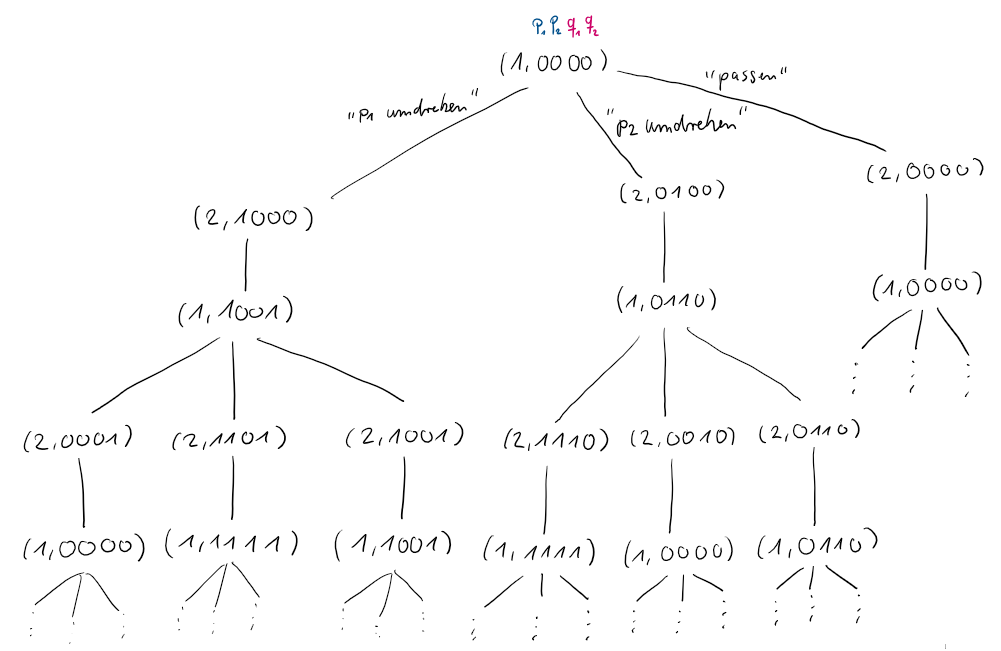
\includegraphics[width=\textwidth]{aufgabe3_gewinnstrategie.png}
\caption{Aufgabe 3b: Gewinnstrategie Spieler 2 }
\label{aufgabe3b}
\end{figure}


\section*{Aufgabe 4)}
-

\section*{Aufgabe 5)}
-


\end{document}
 